% Created 2021-10-02 Sat 10:57
% Intended LaTeX compiler: xelatex
\documentclass[letterpaper]{article}
\usepackage{graphicx}
\usepackage{grffile}
\usepackage{longtable}
\usepackage{wrapfig}
\usepackage{rotating}
\usepackage[normalem]{ulem}
\usepackage{amsmath}
\usepackage{textcomp}
\usepackage{amssymb}
\usepackage{capt-of}
\usepackage{hyperref}
\setlength{\parindent}{0pt}
\usepackage[margin=1in]{geometry}
\usepackage{fontspec}
\usepackage{svg}
\usepackage{cancel}
\usepackage{indentfirst}
\setmainfont[ItalicFont = LiberationSans-Italic, BoldFont = LiberationSans-Bold, BoldItalicFont = LiberationSans-BoldItalic]{LiberationSans}
\newfontfamily\NHLight[ItalicFont = LiberationSansNarrow-Italic, BoldFont       = LiberationSansNarrow-Bold, BoldItalicFont = LiberationSansNarrow-BoldItalic]{LiberationSansNarrow}
\newcommand\textrmlf[1]{{\NHLight#1}}
\newcommand\textitlf[1]{{\NHLight\itshape#1}}
\let\textbflf\textrm
\newcommand\textulf[1]{{\NHLight\bfseries#1}}
\newcommand\textuitlf[1]{{\NHLight\bfseries\itshape#1}}
\usepackage{fancyhdr}
\pagestyle{fancy}
\usepackage{titlesec}
\usepackage{titling}
\makeatletter
\lhead{\textbf{\@title}}
\makeatother
\rhead{\textrmlf{Compiled} \today}
\lfoot{\theauthor\ \textbullet \ \textbf{2021-2022}}
\cfoot{}
\rfoot{\textrmlf{Page} \thepage}
\renewcommand{\tableofcontents}{}
\titleformat{\section} {\Large} {\textrmlf{\thesection} {|}} {0.3em} {\textbf}
\titleformat{\subsection} {\large} {\textrmlf{\thesubsection} {|}} {0.2em} {\textbf}
\titleformat{\subsubsection} {\large} {\textrmlf{\thesubsubsection} {|}} {0.1em} {\textbf}
\setlength{\parskip}{0.45em}
\renewcommand\maketitle{}
\author{David and Jack}
\date{\today}
\title{Emacs Workshop Worksheet}
\hypersetup{
 pdfauthor={David and Jack},
 pdftitle={Emacs Workshop Worksheet},
 pdfkeywords={},
 pdfsubject={},
 pdfcreator={Emacs 28.0.50 (Org mode 9.4.4)}, 
 pdflang={English}}
\begin{document}

\tableofcontents


\section{Intro}
\label{sec:org4650049}

Let's get started making our own configuration file! Make the file \texttt{\textasciitilde{}/.emacs.d/init.el} (remember, you can do that with \texttt{C-x C-f} and typing in the filename). Emacs runs this file whenever you start it.

Emacs is configured in \emph{Emacs Lisp}: so let's quickly review some important parts of Lisp that make it a tad unusual:
\begin{itemize}
\item Everything is \emph{array-based} in Lisp, so instead of calling a function like \texttt{function(arg1, arg2)}, you call it like \texttt{(function arg1 arg2)}
\item Lisp is \emph{functional}, so code does not execute sequentially by default unless for certain circumstances. Code is mostly written by composing functions (nesting function calls).
\item Lisp has a lot of single quotes scattered around: these are not strings but \emph{symbols} that refer to a function/variable by its name. A lot of interfaces in Emacs want the \emph{name} of a function rather than the function itself.
\begin{itemize}
\item Example: \texttt{'(chicken 1)} would not call the function \texttt{chicken} but just return what you literally typed out: that is, \texttt{'(chicken 1)}.
\end{itemize}
\end{itemize}

Let's get started by configuring our first thing! Let's remove those annoying headerbars and scrollbars. \texttt{setq} is a function we're gonna use a lot: it sets the value of a variable (which are used to express most of the options in Emacs). 
\begin{verbatim}
(tool-bar-mode -1) ;; This calls the function tool-bar-mode and turns it off by passing -1
(menu-bar-mode -1) ;; Same but for menubar
(scroll-bar-mode -1) ;; Same but for scroll bar
(setq use-dialog-box nil) ;; Set the variable use-dialog-box to nil, turning off GUI popups
\end{verbatim}

Next we'll banish the horror of \texttt{custom.el} to the abyss. 
\begin{verbatim}
(setq custom-file "/dev/null")
\end{verbatim}

Emacs has a tendency to litter autosave files everywhere, so let's put them all in one place:
\begin{verbatim}
(setq backup-directory-alist `(("." . "~/.saves")))
(setq backup-by-copying t)
\end{verbatim}

We can then load \texttt{package.el} and open ourselves to the Emacs universe!
\begin{verbatim}
(require 'package)
\end{verbatim}

Also we'll set the theme to be \texttt{tango}, but you can change it with  \texttt{M-x load-theme}.
\begin{verbatim}
(load-theme 'tango)
\end{verbatim}


\section{Other Usecases}
\label{sec:org6d2de7f}
\subsection{Binding Keys}
\label{sec:orga727423}
\begin{center}
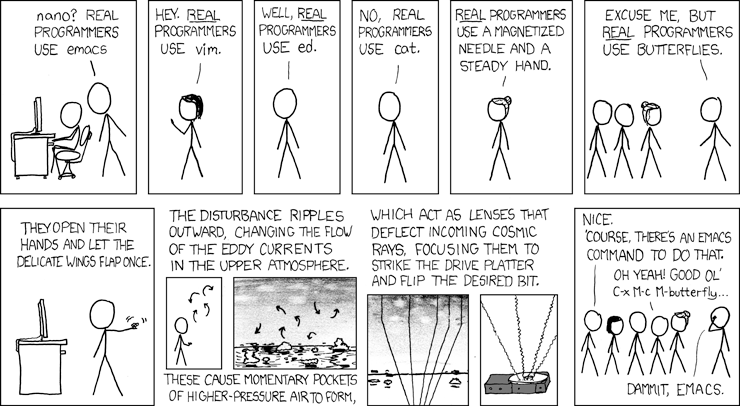
\includegraphics[width=.9\linewidth]{2021-09-27_22-48-23_screenshot.png}
\end{center}

Let's harness the power of the butterfly (although with a shorter key combo)
\begin{verbatim}
(global-set-key (kbd "C-x M-c") 'butterfly)
\end{verbatim}
Now, after evaluating that, use the key combo \texttt{C-x M-c} and unleash Emacs' true potential! 
\subsection{Hooks}
\label{sec:org4d2e393}
Let's say you want to harness the power of the butterfly whenever you open an Emacs Lisp buffer (\textbf{don't actually do this}, since that'll be a bit too much to handle). We can use a \emph{hook}, which allows you to run custom code before/after important events, allowing for a large amount of extensibility. Hooks are actually variables, so if you ever want to search for one, good ol' \texttt{C-h v} will help.
\begin{verbatim}
(add-hook 'emacs-lisp-mode-hook 'butterfly)
\end{verbatim}

This could be use for many other things, like enabling a linter whenever you open a Python buffer.

\section{More Lisp}
\label{sec:org8698e42}

Here's some more complicated examples of plain Emacs Lisp that may not be directly useful just yet.
\begin{verbatim}
(if (> 2 1)
    (message "hello")
  (message "goodbye"))  
\end{verbatim}

\begin{verbatim}
(defun my-function (arg1 arg2)
  (message "look!")
  (message "sequential!")
  (message arg2)
  (message "whee!"))
(my-function "hello" "there")
\end{verbatim}

You also might see something like \texttt{:blah} around, and they're usually for specifying arguments. They're just upgraded string literals, don't worry about them too much.
\end{document}
